% Standalone TikZ diagram: generic NARX structure, drawn to match the Level-3
% network in this paper (narx/model.py).
%
%   taps      state 0,1,2,5 ; throttle 0,1,2,5,10,20 ; rudder 0,1,2,5,10
%   regressor 2*4 + 6 + 5 = 19
%   network   19 -> 64 tanh -> 2
%   output    state increment, added to the current state
%
% Build:  ~/.claude/skills/block-diagram/build.sh narx_architecture.tex

\documentclass[border=4pt]{standalone}
\usepackage{tikz}
\usepackage{amsmath,amssymb}
\usetikzlibrary{positioning, calc, arrows.meta}

\begin{document}
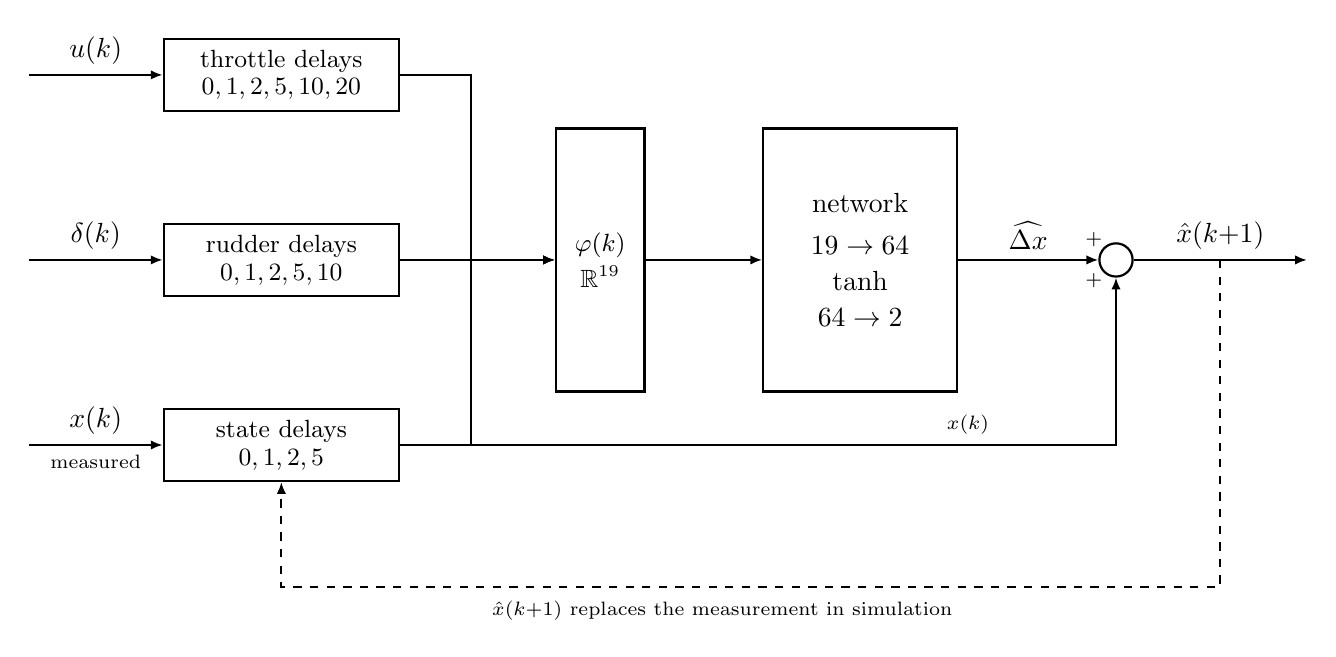
\begin{tikzpicture}[
  >={Latex[length=1.5mm, width=1.2mm]}, thick,
  tap/.style  = {draw, rectangle, minimum height=2.6em, minimum width=8.5em,
                 inner sep=3pt, align=center, font=\small},
  reg/.style  = {draw, rectangle, minimum height=9.5em, minimum width=3.2em,
                 inner sep=3pt, align=center, font=\small},
  net/.style  = {draw, rectangle, minimum height=9.5em, minimum width=7.0em,
                 inner sep=4pt, align=center},
  sum/.style  = {draw, circle, inner sep=0pt, minimum size=1.2em},
]

  % ── tapped delay banks ────────────────────────────────────────────────
  \node[tap] (tu) at (0, 2.35)  {throttle delays\\[-1pt]$0,1,2,5,10,20$};
  \node[tap] (td) at (0, 0)     {rudder delays\\[-1pt]$0,1,2,5,10$};
  \node[tap] (tx) at (0,-2.35)  {state delays\\[-1pt]$0,1,2,5$};

  \coordinate (uin) at ($(tu.west)+(-1.7,0)$);
  \coordinate (din) at ($(td.west)+(-1.7,0)$);
  \coordinate (xin) at ($(tx.west)+(-1.7,0)$);

  \draw[->] (uin) -- node[above]{$u(k)$} (tu);
  \draw[->] (din) -- node[above]{$\delta(k)$} (td);
  \draw[->] (xin) -- node[above]{$x(k)$} node[below, font=\scriptsize]{measured} (tx);

  % ── regressor and network ─────────────────────────────────────────────
  \node[reg] (phi) at (4.05, 0) {$\varphi(k)$\\[2pt]$\mathbb{R}^{19}$};
  \node[net] (net) at (7.35, 0) {network\\[3pt]$19 \rightarrow 64$\\[1pt]$\tanh$\\[1pt]$64 \rightarrow 2$};

  \draw[->] (tu.east) -- ++(0.9,0) |- (phi.west);
  \draw[->] (td.east) -- (phi.west);
  \draw[->] (tx.east) -- ++(0.9,0) |- (phi.west);
  \draw[->] (phi) -- (net);

  % ── increment added to the current state ──────────────────────────────
  \node[sum] (sum) at (10.6, 0) {};
  \coordinate (xout) at ($(sum.east)+(2.2,0)$);

  \node[font=\scriptsize, inner sep=0pt, anchor=south east] at (sum.north west) {$+$};
  \node[font=\scriptsize, inner sep=0pt, anchor=north east] at (sum.south west) {$+$};

  \draw[->] (net) -- node[above]{$\widehat{\Delta x}$} (sum);
  \draw[->] (sum) -- node[above]{$\hat x(k{+}1)$} (xout);

  % current state joins the increment, routed below the network blocks
  \coordinate (xbr) at ($(tx.east)+(0.55,0)$);
  \draw[->] (xbr) -- node[pos=0.78, above, font=\scriptsize]{$x(k)$} (xbr -| sum) -- (sum.south);

  % ── feedback: the loop that only closes in simulation ─────────────────
  \coordinate (fbk) at ($(sum.east)!0.5!(xout)$);
  \draw[->, dashed] (fbk) -- ++(0,-4.15) -| (tx.south);
  \node[font=\scriptsize, align=center] at (5.6,-4.45)
        {$\hat x(k{+}1)$ replaces the measurement in simulation};

\end{tikzpicture}
\end{document}
